\documentclass[a4paper,UTF8]{article}
\usepackage{ctex}
\usepackage[margin=1.25in]{geometry}
\usepackage{color}
\usepackage{graphicx}
\usepackage{amssymb}
\usepackage{amsmath}
\usepackage{amsthm}
%\usepackage[thmmarks, amsmath, thref]{ntheorem}
\theoremstyle{definition}
\newtheorem*{solution}{Solution}
\newtheorem*{prove}{Proof}
\usepackage{multirow}
\usepackage{url}
\usepackage{enumerate}
\usepackage{listings}
\usepackage{caption}
\usepackage{subfigure}
\usepackage[colorlinks,linkcolor=black, anchorcolor=black,citecolor=black,]{hyperref}


\begin{document}
\title{\textbf{《计算机图形学》十一月报告}}
\author{学号:181860077 姓名:佘帅杰,\href{mailto:3121416933@qq.com}{3121416933@qq.com}}
\maketitle

\section{综述}
注:本次报告是增量式的报告,即本次的报告内内容就是这个月做的内容\\
在上个月已经基本实现了算法部分的内容,这个月的工作主要可以概括到下面的四个方面
\begin{enumerate}
    \item 着手阅读GUI的框架代码
    
    \item 着手阅读pyQT相关的模块和接口
    
    \item 着手实现GUI相关的功能
    
    \item 修改遇到的算法模块的BUG
\end{enumerate}

目前已经实现的GUI部分
\begin{enumerate}
    \item 绘制直线,椭圆,多边形。
    
    \item 利用鼠标选中图元
    
    \item 平移,旋转
    
    \item 保存和清空画布
    
    \item 选择画笔颜色
\end{enumerate}
\section{GUI框架介绍}
\subsection{概述}
GUI框架主要是由如下的三个部分组成的

\begin{enumerate}
    \item MyCanvas:主要是画布,负责管理各个图元以及和监管鼠标的操作,会根据鼠标
    的操作已经当前的状态做对应的反应
    
    \item MyItem:作为基本的图元单位,保存了图元的信息以及图元的最基本的操作
    比如绘制自己和他的选中框
    
    \item MainWindow:作为相对上层的一个结构,主要负责的就是管理下游的图元
    更多的他代表了外层的窗口管理,负责和一些鼠标对菜单的操作的响应
\end{enumerate}

\subsection{具体函数分析}
\subsubsection{MyCanvas}
start\_draw\_line类似的函数主要就是负责绘制,但是这里的绘制并不是真正的绘制
在画布上的绘制,而是开始准备绘制色湖之状态位,在每一次的刷新才会根据Item自己的操作
进行绘制和显示。

以mouse打头的操作一般都是上文提到的对鼠标的操作进行响应的操作,包括鼠标的按下
移动以及松开,对应的在绘制里就是开始记录坐标点的时机。对于鼠标的按下还需要根据当前的
状态看看是不是选中图元之类的操作

\subsubsection{MyItem}
最基本的图元单位,保存了图元的相关信息,这里并不是直接保存了所有的绘制点,而是
保存了图元绘图的所需信息,即前面实现算法的时候需要的参数

有了上面保存好的参数之后就可以开始绘制,其中paint函数会做相关的操作,主要
的操作就是对每一个像素点draw,这个和QGraphicItem的内置有一些关系。

然后每一次除了画出自身之外还要记得看看自己是不是被选中了,如果是被选中的记得要把选中
框也要画出来,同时观察到这里绘制选中框设置设置了画笔的颜色,对应的可以实现
需求里的设置画笔的功能

\subsubsection{MainWindow}
这个类继承了QMainWinodow,同时在一开始的init里就有大量的设置的操作。
基本是在构造窗口的结构,以及设置按钮和绑定按钮和函数,涉及到了一些信号槽的
理念,此处略过。

各种以Action结尾的函数是作为按下按钮后的对应执行函数,主要做的事就是在和窗口
交互以及位Canvas的操作提供条件,基本的事件总结一下就是设置一下状态栏显示的
文字,然后调用对应canvas执行操作



\section{具体实现}
上面的解释是初步的在实现之前对框架代码的阅读理解,下面是具体的开发

\subsection{绘制直线}
对直线的绘制是相对简单的,因为有一个Naive作为基础,只需要类比,把
各种的函数调用换一下就行,这里省略不赘述,具体的实现思路和下面对于
椭圆绘制的实现相似

\subsection{绘制椭圆}
椭圆的绘制,根据日常的使用可以知道,在GUI里的期望动作就是可以点击鼠标,然后拖动
鼠标,鼠标停下的位置和一开始点击的位置是两个边界点,最终的椭圆就生成于这两个点
之间,同时在拖动的过程里可以看到椭圆变大变小从而便于观察和调整绘制的大小

所以结合之前对代码的观察,主要的实现步骤如下
\begin{enumerate}
    \item 增加椭圆相关的信号槽绑定
    
    \item 在MainWindow里添加相关的Action函数
    
    \item 进一步的就跳转到了start\_draw\_ellipse,把当前的状态设置好,然后选中
    当前的id,由于椭圆只有中点圆绘制一种算法,所以不需要指定算法的参数设定

    \item 接下来自然用户会开始操作鼠标,准备绘制,于是对应的在mousePressEvent
    函数中实现对应的功能,按下鼠标说明用户铁了心要画椭圆,于是根据刚才的状态
    进行判断,认为要画椭圆则生成对应的图元单位,然后放在列表里

    \item 刚才提到了随着鼠标的移动,待定的椭圆也要跟着变化,同时谁也不知道用
    户什么时候就不动然后松开鼠标,所以每次鼠标的移动都要保存下最后的位置,也就是
    把控制点(plist)的第二点设置为移动的位置,则代码就会做当前位置的绘制
    
    \item 截至到这里,基本椭圆的绘制GUI实现就已经做好了,其他的细节略
\end{enumerate}

\begin{figure}[h]
	\centering
	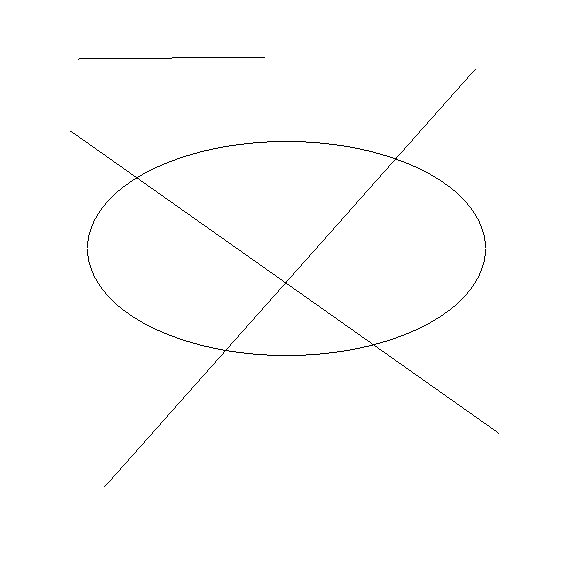
\includegraphics[scale=0.3]{figure/EillpsGUI.png}
	\caption{EillpsGUI效果图图}
	\label{fig:EillpsGUI}
\end{figure}


\subsection{绘制多边形}
多边形的绘制相对的会复杂一些,多边形是由多条边组成的,初步的设计是让鼠标的左键
不断的点击(拖动)选中新坐标点,然后鼠标右键表示作画结束,因此基本的实现思路就是
不断的捕获左键的操作,然后把坐标点加入p\_list。

注意到在作画结束之前,图形不一定是封闭的,于是原先写好的多边形绘制算法并不能
直接使用,因此对应的做了一些修改,封装到draw\_polygoning函数,取消了最后一个
点和第一个点的练接,直到捕获到右键之后说明作画结束,才会调用原来的绘制多边形函数

\begin{figure}[h]
	\centering
	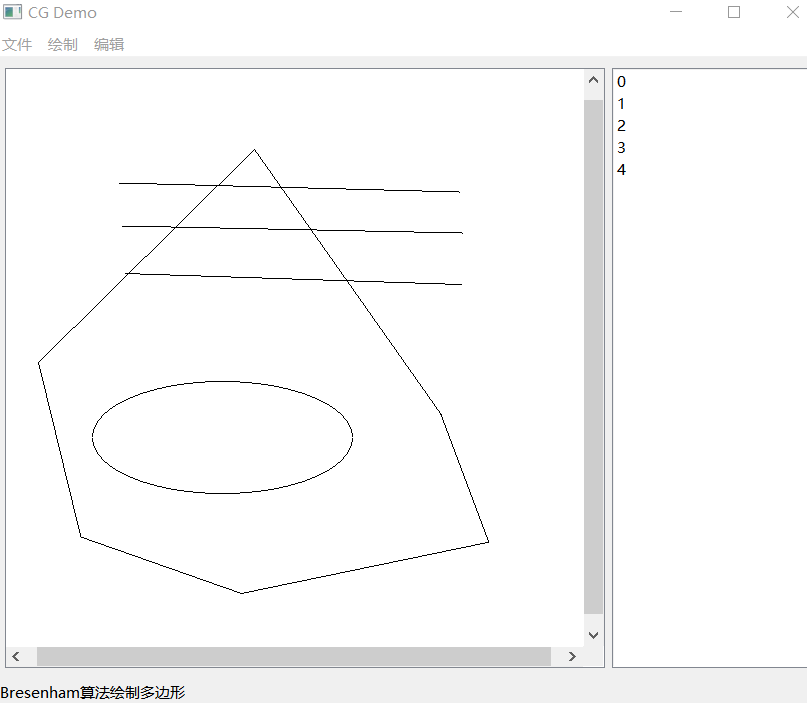
\includegraphics[scale=0.4]{figure/draw.png}
	\caption{绘图算法效果图}
	\label{fig:DrawGUI}
\end{figure}

\subsection{画笔设置}
之前已经提到了,框架代码在绘制的时候加上了设置颜色的操作,同理我可以在一开始的
时候设置在菜单里让用户选择对应的颜色,等到用户选择好了颜色之后,我在类里加上
一个变量专门记录一下这个选择的结构,然后在Item每一次绘制的时候都提醒Item使用
对应的颜色作画。

实现流程实际上和上述实现椭圆的过程是差不多,都是要从MainWindow开始入手,先
修改菜单的结构,然后Connect信号和槽,接着在Canvas里和item里对应实现即可,自身
没有太大的技术需求

比较有意思的就是用到了Qt提供的一个QColorDialog,能够直接显示出选择颜色的颜色盘

\begin{figure}[h]
	\centering
	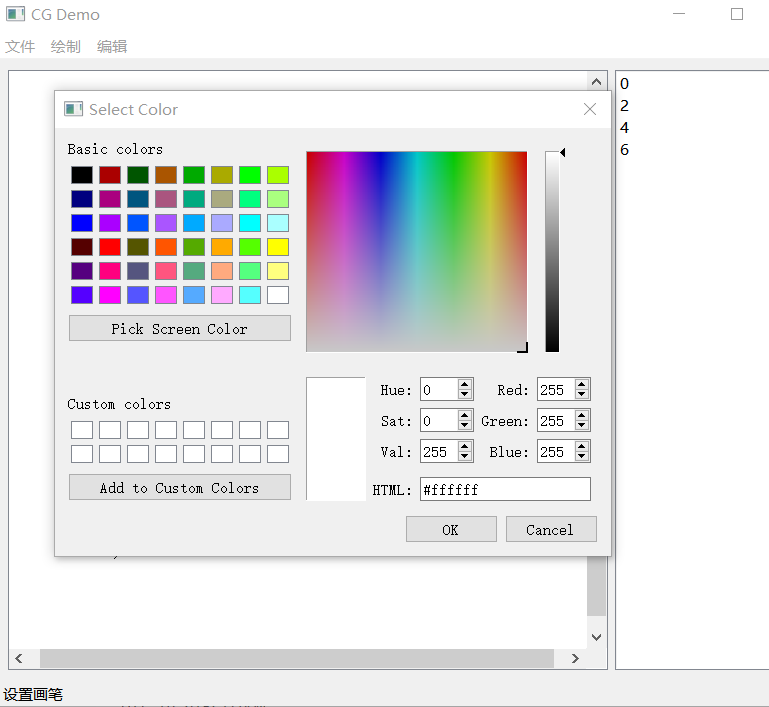
\includegraphics[scale=0.3]{figure/ChooseColor.png}
	\caption{设置画笔效果图}
	\label{fig:EillpsGUI}
\end{figure}


\subsection{保存图元}
实现保存图元,基本的操作和上面都是一样的,从定义菜单到槽函数等等
比较不一样的自然就是保存,怎么才可以把所有的绘制图元拔下来放进图片?
使用的是QGraphicsView里的grab来保存。然后QT中dialog提供了选择文件保存的
界面接口对话框:dialog.getSaveFileName。最后的实现效果基本如下

\begin{figure}[h]
	\centering
	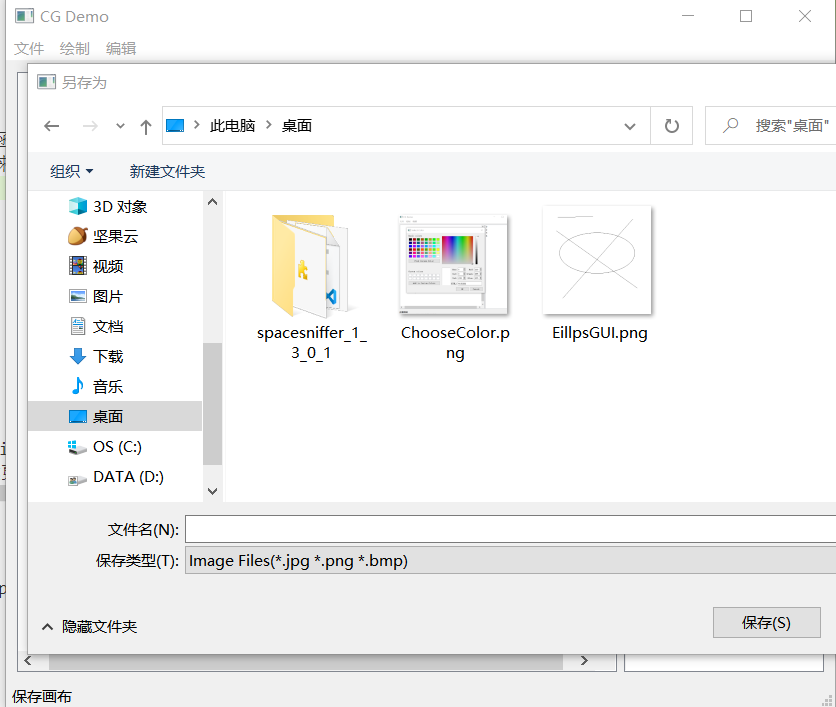
\includegraphics[scale=0.5]{figure/SaveCanvas.png}
	\caption{保存界面示意图}
	\label{fig:SaveCanvas}
\end{figure}

以及最后保存的结果(输入的文件名就是test)
\begin{figure}[h]
	\centering
	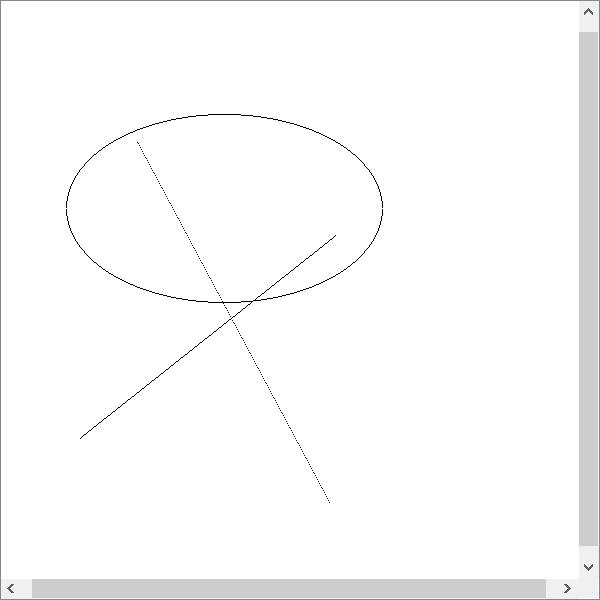
\includegraphics[scale=0.5]{figure/test.jpg}
	\caption{保存画布结果图}
	\label{fig:SaveCanvas}
\end{figure}

\subsection{BUG修复}
在进一步的实现GUI的时候发现了一些BUG,随后进行了修复

\subsubsection{曲线绘制算法BUG}
之前的曲线绘制没有考虑到左右两个端点是同一个点的情况,同样在测试样例里也没有这样
但是在GUI的使用的时候,由于椭圆是随着鼠标的移动而绘图的,所以这个时候一开始会出现左右两个端点在同一个位置的情况
进一步的触发了BUG,发现这个BUG后进行修改,在计算之前就先加入左右端点即可

 
\section{系统介绍}
目前的CG2020图形学系统已经支持
\begin{itemize}
    \item 命令行和GUI界面调用直线生成算法
    \item 命令行调用多边形生成算法和中点圆生成算法
    \item 在GUI界面中使用鼠标直接的选中所需图元
    \item 命令行调用曲线生成算法,可选算法Bezier和B-spline
    \item 在命令行调用指令,对图元做平移,旋转,缩放,裁剪操作
    \item 在GUI界面绘制直线,多边形,椭圆
    \item 在GUI界面操作图元平移
    \item 在GUI界面调整画笔
    \item 在GUI界面保存画布
\end{itemize}

\section{总结}
本次实验主要是对GUI的框架代码进行了相对深入的了解,在了解的同时
逐步的开展相应的功能实现,主要围绕着绘图和绘图相关的实用功能。
在实现的同时,检测和挖掘先前算法实现的种种BUG并修复


\bibliography{xxx}

\begin{thebibliography}{99}  
    \bibitem{ref1}《计算机图形学教程》孙正兴编 
    \bibitem{ref2} \href{https://www.google.com/imghp?hl=zh-CN&ogbl}{Google图片}
    \bibitem{ref3} \href{https://build-system.fman.io/pyqt5-tutorial}{PyQT5 Tutorial}
    
\end{thebibliography}

\end{document}

\bibliographystyle{plain}